\chapter{Tinjauan Pustaka dan Dasar Teori}

\section{Tinjauan Pustaka}

Penelitian tentang pengembangan sistem informasi untuk mengelola data penelitian dan PkM 
telah banyak dilakukan oleh berbagai peneliti. Berikut ini merupakan beberapa penelitian 
terkait yang dilakukan oleh peneliti lain.

Sri Handayani pernah melakukan penelitian tentang perancangan sistem informasi penelitian dan
PkM berbasis web untuk Fakultas Teknologi Informasi dan Komunikasi (FTIK) Universitas Semarang(USM). Penelitian tersebut bertujuan untuk
meningkatkan keakuratan dan integrasi data penelitian dan PkM di Fakultas Teknologi Informasi dan Komunikasi (FTIK) Universitas Semarang. Ketidakakuratan data 
penelitian dan PkM terjadi karena terkadang terdapat perbedaan data dari pihak program studi, 
fakultas, maupun LPPM. Perancangan sistem informasi menggunakan arsitektur
MVC (\textit{Model View Controller}) yang memisahkan antara tampilan, logika bisnis, dan basis data
Teknologi yang digunakan yaitu menggunakan \textit{framework} CodeIgniter dan \textit{database} MySQL.
Hasil dari penelitian tersebut adalah sistem informasi yang dapat menjalankan tiga fungsi utama
yaitu pendataan, transaksi, dan pelaporan. Proses pendataan yaitu proses pada saat dosen melakukan 
registrasi untuk mengikuti penelitian atau PkM. Proses transaksi yaitu proses dosen mengisi
catatan harian saat sedang dalam masa pelaksanaan penelitian atau PkM. Proses pelaporan yaitu
pada saat dosen melakukan upload dokumen usulan, laporan kemajuan, dan laporan akhir\cite{handayani_rancang_nodate}.

Desi Ratnasari pernah melakukan penelitian tentang perancangan sistem informasi penelitian dan
PkM berbasis web untuk LPPM STT Terpadu Nurul Fikri. Penelitian tersebut bertujuan untuk 
membangun sistem informasi untuk penyusunan laporan, serta pencarian dan pengelolaan data 
penelitian dan pengabdian kepada masyarakat. Sistem informasi tersebut berguna untuk 
meningkatkan integritas dan keamanan data penelitian dan PkM di LPPM STT Terpadu Nurul Fikri,
dimana sebelumnya, pengelolaan data masih dilakukan secara manual menggunakan Microsoft Excel dan Word. 
Perancangan sistem Informasi tersebut menggunakan \textit{framework} Yii2 dan \textit{database} MySQL.
Tahapan penelitian yang dilakukan yaitu analisis sistem, desain sistem, implementasi 
\textit{code} program, pengujian, dan pemeliharaan. Hasil dari penelitian ini yaitu sistem 
informasi penelitian dan pengabdian kepada masyarakat dengan fitur untuk mengelola surat 
pengajuan, pengsahan, tugas, dan keabsahan, serta mengelola anggota, BSCHP, dan anggaran\cite{ratnasari_analisis_2017}.

Sopiyan Dalis pernah melakukan penelitian mengenai perancangan sistem informasi penelitian 
dan pengabdian kepada masyarakat berbasis web untuk LPPM Akademik Bina Sarana Informatika(BSI). 
Sistem informasi tersebut dirancang untuk mempercepat kinerja LPPM Akademik 
BSI dalam mengelola data penelitian dan pengabdian kepada masyarakat, serta 
berita atau informasi dari luar universitas karena sebelumnya masih dilakukan 
secara manual menggunakan Microsoft Excel dan Word, dan pengiriman dokumen surat melalui \textit{email}. 
Metode yang digunakan yaitu \textit{Software Development Life Cycle} (SDLC) \textit{waterfall} 
dengan tahapan analisa kebutuhan, desain, \textit{code} program, pengujian, dan 
\textit{maintenance}. Teknologi yang digunakan yaitu menggunakan bahasa PHP dan 
\textit{database} MySQL\cite{dalis_rancang_2017}. 

Hajir Rummujib dam Pariuyadi pernah melakukan penelitian mengenai perancangan 
aplikasi penelitian dan pengabdian kepada masyarakat berbasis \textit{mobile} 
untuk LPPM Universitas Nurdin Hamzah. Penelitian tersebut bertujuan untuk 
membuat sistem informasi dan manajemen yang mengedepankan kemudahan dalam 
pengelolaan data dan pemberitahuan informasi mengenai penelitian dan pengabdian
kepada masyarakat. Sistem informasi tersebut dikembangkan menggunakan  
flutter untuk \textit{front-end}, PHP untuk \textit{back-end}, dan MySQL sebagai \textit{database}\cite{rummujib_aplikasi_1907}. 

Goesderilidar pernah melakukan penelitian mengenai pearncangan web LPPM Sekolah Tinggi 
Manajemen dan Ilmu Komputer (STMIK) Indragiri. Perancangan web ini bertujuan 
untuk memudahkan dosen dalam melaporkan penelitian dan pengabdian kepada 
masyarakat. Web tersebut dibuat menggunakan \textit{platform} permbuatan 
\textit{website} yaitu Wordpress\cite{__membangun_2021}.


Berisi tugas akhir-tugas akhir terdahulu yang terkait dengan judul skripsi yang dilakukan. Hal ini meliputi skripsi, tesis, atau publikasi terdahulu yang terkait dengan judul skripsi yang diusulkan. Lakukan pembahasan secara sistemastis dengan menjelaskan masalah apa yang dilakukan oleh tugas akhir terdahulu, kontribusi yang dilakukan, serta analisis penulis terkait dengan keunggulan dan keterbatasan tugas akhir. 

Setelah membahas berbagai tugas akhir terdahulu, maka alangkah baiknya penulis melakukan rangkuman terutama terkait dengan peluang pengembangan atau tugas akhir yang akan dilakukan.


\section{Dasar Teori}

Berisi teori-teori yang menjadi dasar solusi atau produk hasil skripsi. Dasar teori pada umumnya diperoleh melalui buku referensi, publikasi tugas akhir, dan informasi web yang dapat dipertanggungjawabkan. Hindari penggunaan dasar teori melalui tautan wikipedia, surat kabar, atau portal berita.

\subsection{Sistem Informasi}
Menurut Robert A. Leitch dan K. Roscoe Davis, sistem informasi adalah suatu sistem di dalam 
suatu organisasi yang memenuhi kebutuhan pemrosesan transaksi sehari-hari, mendukung operasi, 
mewakili aktivitas manajerial dan strategis organisasi, dan menyediakan laporan yang 
diperlukan kepada pihak eksternal tertentu\cite{ratnasari_analisis_2017}. Sistem informasi juga dapat diartikan sebagai
suatu sistem yang mengambil data lalu mengolahnya menjadi informasi yang berguna bagi
pengguna. 

\subsection{Aplikasi Web}
Aplikasi web merupakan \textit{software} atau aplikasi yang diakses melalui aplikasi 
\textit{browser}, seperti Google Chrome, Mozilla Firefox, Safari, dan sebagainya, melalui 
internet. \cite{jazayeri_trends_2007}. Berbeda dengan aplikasi 
\textit{desktop} ataupun \textit{mobile}, aplikasi web dapat diakses melalui berbagai 
perangkat,seperti laptop, \textit{smartphone}, dan \textit{tablet}, tanpa harus menginstall 
aplikasi tersebut terlebih dahulu. Selain itu, \textit{content} yang disediakan pada web 
aplikasi lebih \textit{update} daripada aplikasi \textit{desktop} yang harus dilakukan \textit{update} 
secara manual agar mendapatkan \textit{content} yang terbaru.  

Berbeda dengan website statis pada umumnya, aplikasi web memiliki fitur yang lebih kompleks. 
Aplikasi web dituntut untuk dapat memenuhi kebutuhan pengguna melalui berbagai fungsi yang 
ditawarkan. Aplikasi web didesain bersifat interaktif terhadap penggunanya atau bersifat dua 
arah, sehingga pengguna tidak hanya mendapatkan data atau informasi saja, melainkan juga dapat 
melakukan manipulasi data seperti mengubah, menambah, dan menghapus data. Pada umumnya, 
aplikasi web juga menerapkan \textit{authentication \emph{dan} authorization} 
untuk keamanan dalam memanipulasi data yang bersifat personal\cite{geeksforgeeksDifferenceBetween}. 


\subsection{MERN \textit{Stack Development}}

MERN merupakan singkatan dari MongoDB, Express JS, ReactJs, NodeJs. 
MERN adalah \textit{stack} pengembangan aplikasi web yang terdiri dari empat 
teknologi utama yaitu MongoDB sebagai \textit{database}, ExpressJS sebagai \textit{framework} 
yang berjalan di atas NodeJS, ReactJS sebagai pustaka JavaScript untuk bagian \textit{User Interface}, 
dan NodeJS sebagai lingkungan \textit{runtime} JavaScript yang berjalan di sisi \textit{server} 
seperti yang ditunjukkan pada Gambar \ref{Fig:mern_visualization}. 
MERN merupakan \textit{stack} pengembangan aplikasi web yang populer karena fleksibilitas dan 
kemudahan dalam mengembangkan aplikasi web. MERN bersifat \textit{open source} 
sehingga dapat dikembangkan dan digunakan secara gratis oleh siapapun. MERN juga memiliki 
komunitas yang besar, di mana para \textit{developer} dapat berbagi pengalaman dan 
pengetahuan mengenai pengembangan aplikasi web menggunakan MERN. Terdapat kesamaan dalam 
teknologi MERN yaitu keempat teknologi tersebut menggunakan bahasa pemrograman JavaScript, 
sehingga jika ingin mengembangkan aplikasi web menggunakan MERN, \textit{developer} hanya
perlu menguasai satu bahasa pemrograman saja sebagai landasan\cite{badru_mern_2022}.

\begin{figure}[h]
	\centering
	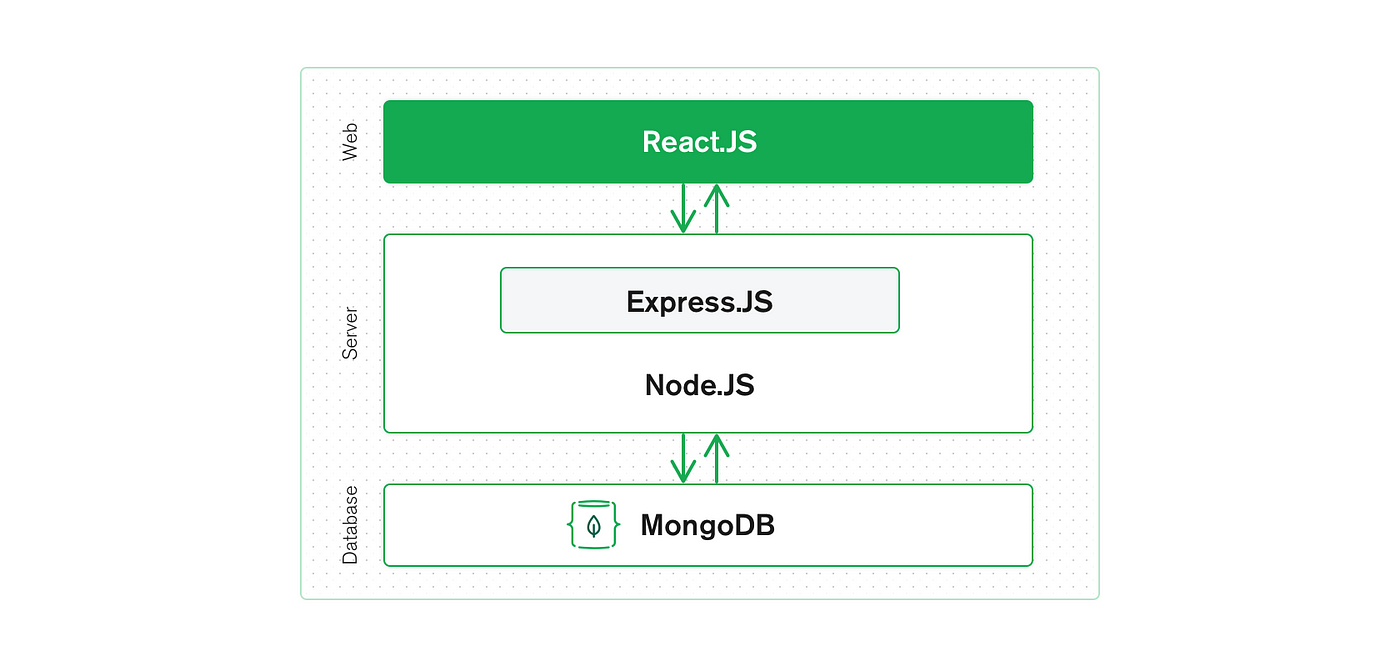
\includegraphics[width=12cm]{contents/chapter-2/mern_visualization.png}
	\caption{Diagram arsitektur \textit{stack} teknologi MERN \cite{s_what_2021}}
	\label{Fig:mern_visualization}
\end{figure}


Pada \textit{stack} teknologi MERN, MongoDB berperan sebagai \textit{database} untuk 
menyimpan data aplikasi web. MongoDB merupakan \textit{database} yang termasuk dalam kategori 
\textit{database} NoSQL yang bersifat \textit{document-oriented} dimana data disimpan dalam
bentuk kumpulan dokumen. Dokumen pada MongoDB disimpan dalam format BSON atau Binary JSON (\textit{JavaScript Object Notation})
yang terdiri dari pasangan \textit{key-value}. MongoDB bersifat \textit{schemaless} yang berarti
tidak memerlukan skema atau struktur yang tetap untuk setiap dokumen yang disimpan. 
Hal ini memudahkan \textit{developer} dalam mengembangkan aplikasi web karena tidak perlu
mengubah struktur \textit{database} jika terjadi perubahan pada aplikasi web. 
MongoDB memiliki fitur \textit{aggregation} yang memungkinkan \textit{developer} untuk
melakukan operasi agregasi seperti \textit{grouping, filtering, dan sorting} pada data yang
disimpan. MongoDB juga memiliki fitur \textit{indexing} yang memungkinkan \textit{developer} untuk
mengoptimalkan proses pencarian data pada \textit{database} \cite{boicea_mongodb_2012}. 
Dalam hal skalabilitas, MongoDB memiliki fitur \textit{sharding} yang memungkinkan \textit{developer} untuk 
membagi data menjadi beberapa bagian dan menyimpannya pada beberapa \textit{server} yang berbeda, 
sehingga dapat mengukur kapasitas aplikasi web yang dikembangkan\cite{kookarinrat_analysis_2015}

Pada \textit{stack} teknologi MERN, ExpressJS berperan sebagai \textit{framework} yang berjalan di atas NodeJS. 
ExpressJS Dicipptakan oleh TJ Holowaychuk pada tahun 2010\cite{vu_building_2020}. ExpressJS merupakan \textit{framework} yang 
bersifat \textit{unopinionated} yang berarti \textit{framework} ini tidak memiliki aturan atau struktur yang 
baku dalam mengembangkan aplikasi web\cite{lakshmi_website_2023}. Hal ini memungkinkan \textit{developer} untuk menentukan sendiri 
struktur aplikasi ExpressJS yang akan digunakan untuk mengembangkan aplikasi web. 
ExpressJS juga berbagai macam \textit{middleware} yang memungkinkan \textit{developer} 
untuk menambahkan fitur-fitur baru pada aplikasi web yang dikembangkan. ExpressJS juga memiliki 
\textit{routing} yang memungkinkan \textit{developer} untuk menentukan rute atau alamat URL yang akan 
diakses oleh pengguna. ExpressJS juga memiliki \textit{templating engine}, seperti Jade Engine, yang memungkinkan \textit{developer} 
untuk mengembangkan aplikasi web yang bersifat \textit{server-side rendering}\cite{jiang_architecture_2015}.

Pada \textit{stack} teknologi MERN, ReactJS berperan sebagai pustaka JavaScript untuk bagian \textit{User Interface} 
yang dikembangkan oleh Facebook. ReactJS menggunakan prinsip \textit{component-based} yang memungkinkan \textit{developer} 
untuk mengembangkan aplikasi web dengan membagi aplikasi web menjadi beberapa komponen yang dapat digunakan 
kembali. Hal ini memudahkan \textit{developer} dalam mengembangkan aplikasi web karena dapat mengurangi 
jumlah kode yang ditulis. Selain itu, penggunaan komponen juga dapat mengurangi waktu saat proses 
\textit{debugging} karena \textit{developer} hanya perlu mencari kesalahan pada komponen yang bermasalah.
ReactJS juga memiliki \textit{virtual DOM} yang memungkinkan \textit{developer}
untuk mengubah tampilan aplikasi web secara dinamis tanpa harus melakukan \textit{refresh} pada halaman web\cite{dinku_reactjs_2022}. 
ReactJS menggunakan state dan props untuk mengatur data yang akan ditampilkan pada aplikasi web. 
State merupakan data yang bersifat dinamis yang dapat berubah-ubah sesuai dengan kondisi aplikasi web. 
Props merupakan data yang bersifat statis yang tidak dapat berubah-ubah.

Pada \textit{stack} teknologi MERN, NodeJS berperan sebagai \textit{runtime environment} yang 
dikembangakn oleh Ryan Dahl pada tahun 2009. NodeJS memungkinkan kode JavaScript berjalan di luar \textit{browser} yaitu di sisi \textit{server}. 
NodeJS menggunakan \textit{event-driven} dan \textit{non-blocking I/O} yang memungkinkan NodeJS 
untuk menjalankan kode secara asinkronus. Hal ini memungkinkan NodeJS untuk menjalankan kode 
yang membutuhkan waktu yang lama tanpa harus menunggu kode tersebut selesai dijalankan. 
NodeJS juga memiliki \textit{package manager} yang bernama NPM (\textit{Node Package Manager}) 
yang memungkinkan \textit{developer} untuk mengunduh dan menginstal \textit{package} yang dibutuhkan 
untuk mengembangkan aplikasi web. \cite{rimal_developing_2019}

\subsection{Material UI}
Material UI adalah \textit{library} ReactJS yang berisi komponen-komponen yang dibuat berdasarkan Material Design 
yang dikembangkan oleh Google\cite{mannila_sales_2022}. Material UI menyediakan berbagai macam komponen React yang \textit{reusable}
yang dapat digunakan untuk mengembangkan aplikasi web. Material UI juga menyediakan dokumentasi yang lengkap 
mengenai komponen-komponen yang mereka sediakan, seperti \textit{button, icon, list, \emph{dan}dropdown},
serta bagaimana mengimplementasikannya pada aplikasi React yang sedang dikembangkan. 
Material UI juga memiliki \textit{theme} yang mempermudah \textit{developer} 
dalam mengkonfigurasi tema yang akan digunakan, seperti warna, ukuran, dan jenis font. 
Karena merupakan \textit{library} React, komponen-komponen tersebut memiliki \textit{style} 
penulisan kode yang sama seperti ReactJS, sehingga \textit{developer} yang sudah terbiasa 
menggunakan ReactJS tidak akan kesulitan dalam menggunakan Material UI.

\subsection{Json Web Token}
Menurut Website resminya, Json Web Token (JWT) adalah standar terbuka (RFC 7519) yang mendefinisikan cara untuk 
mengirimkan informasi secara aman antar pihak menggunakan objek JSON. Dalam pengembangan 
aplikasi web, JWT digunakan untuk mengautentikasi pengguna yang mengakses aplikasi. 
JWT terdiri dari tiga bagian, yaitu \textit{header, payload,} dan \textit{signature} seperti 
yang terlihat pada Gambar \ref{Fig:Struktur_JWT}.
\textit{Header} berisi informasi mengenai algoritma enkripsi yang digunakan untuk mengenkripsi \textit{payload}. 
\textit{Payload} berisi informasi pengguna yang akan digunakan untuk mengakses aplikasi web. 
\textit{Signature} berisi hasil enkripsi dari \textit{header} dan \textit{payload} menggunakan algoritma yang 
didefinisikan pada \textit{header}. Kemudian, ketiga bagian tersebut digabung dan di-\textit{encode} 
menjadi token string random yang sulit untuk dihapal.

\begin{figure}[h]
	\centering
	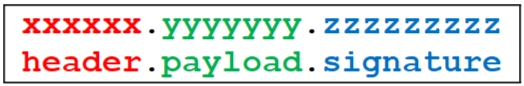
\includegraphics[width=6cm]{contents/chapter-2/struktur_jwt.jpg}
	\caption{Struktur JWT \cite{rahmatulloh_keamanan_2018}} 
	\label{Fig:Struktur_JWT}
\end{figure}

Salah satu kegunaan JWT pada suatu aplikasi web adalah untuk mengautentikasi \textit{user} yang mengakses aplikasi web. 
Pada saat \textit{user} melakukan \textit{login}, \textit{server} akan mengirimkan token JWT ke aplikasi web. 
Setelah itu, aplikasi web akan menyimpan token JWT pada \textit{local storage} atau \textit{session storage}. 
Token itulah yang harus disertakan setiap kali \textit{user} mengakses halaman web dan \textit{request resource \emph{dari} server}. 
Token tersebut akan dikirimkan ke \textit{server} untuk diverifikasi. Jika token tersebut valid, 
\textit{server} akan mengirimkan \textit{resource} yang diminta oleh \textit{user}. Gambar \ref{Fig:JWT_works} 
menunjukkan bagaimana JWT bekerja dalam mengautentikasi \textit{user} yang mengakses aplikasi web.

\begin{figure}[h]
	\centering
	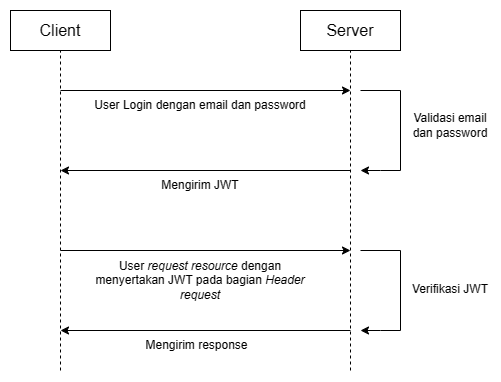
\includegraphics[width=9cm]{contents/chapter-2/jwt_works.png}
	\caption{Sequence diagram autentikasi JWT}
	\label{Fig:JWT_works}
\end{figure}


\subsection{Cloudinary}

Cloudinary merupakan suatu \textit{platform} manajemen media berbasis \textit{cloud} 
yang menyediakan solusi dalam penyimpanan, pengoptimalan, dan pengiriman file media 
seperti gambar, dokumen, video, dan audio\cite{ayuningtyas2017undangan}. Cloudinary 
memiliki berbagai fitur untuk menyederhanakan proses manajemen dan manipulasi 
aset media. Fitur-fitur tersebut dapat menjadi solusi bagi para 
\textit{software developer} dalam memanajemen file media pada aplikasi yang 
mereka kembangkan. Untuk memudahkan penggunanya, platform ini menyediakan 
dokumentasi yang lengkap mengenai berbagai layanan yang mereka tawarkan serta 
bagaimana cara menggunakannya. Cloudinary juga memiliki fleksibilitas yang 
baik dalam mendukung proses \textit{software development} karena API yang 
disediakan dapat terintegrasi dengan berbagai macam \textit{framework}, baik 
\textit{back-end, front-end, \emph{maupun} mobile} seperti yang terlihat pada
Gambar \ref{Fig:cloudinary_framework}, yang terdapat pada situs resminya\cite{cloudinary-website}.

\begin{figure}[h]
	\centering
	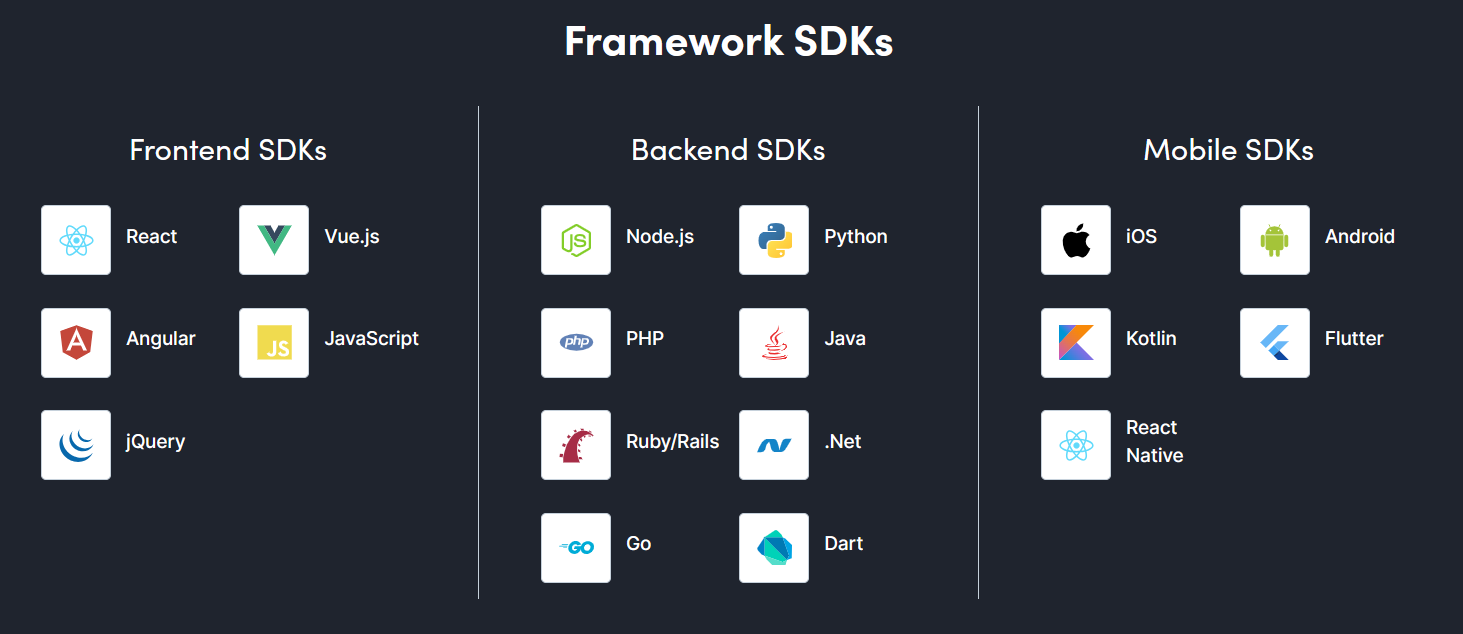
\includegraphics[width=12cm]{contents/chapter-2/cloudinary_framework.png}
	\caption{\textit{Framework} yang didukung oleh Cloudinary \cite{cloudinary-website}}
	\label{Fig:cloudinary_framework}
\end{figure}

% \subsection{\textit{Entity Relationship Diagram}(ERD)}


% \subsection{\textit{Use Case Diagram}}
% \textit{Use case diagram} adalah diagram yang menggambarkan interaksi antara \textit{user} dengan sistem yang dibuat. 
% \textit{Use case diagram} terdiri dari \textit{actor, use case,} dan \textit{relationship}. 
% \textit{Actor} adalah entitas yang berinteraksi dengan sistem. \textit{Use case} adalah 
% fungsi-fungsi yang dapat dilakukan oleh \textit{actor}. \textit{Relationship} adalah 
% hubungan antara \textit{actor} dan \textit{use case}. Gambar \ref{Fig:Use_Case_Diagram}
% menunjukkan \textit{use case diagram} dari aplikasi yang dibuat. 
\subsection{Metode Pengembangan \textit{Software}}
Dalam mengembangkan suatu aplikasi atau \textit{software}, terdapat beberapa metode yang dapat digunakan. 
Metode tersebut dapat digunakan untuk mengatur proses pengembangan \textit{software} agar dapat 
dilakukan dengan lebih terstruktur dan terarah. Dalam dunia \textit{software development}, metode 
pengembangan \textit{software} dikenal dengan sebutan \textit{software development life cycle} (SDLC). 
SDLC adalah suatu proses yang terstruktur untuk mengembangkan \textit{software} yang terdiri dari 
beberapa tahapan. Tahapan-tahapan tersebut dapat disesuaikan dengan kebutuhan dan karakteristik 
dari \textit{software} yang akan dikembangkan. Pada bagian ini, akan dijelaskan mengenai 
dua metode SDLC yang dapat digunakan dalam mengembangkan \textit{software} yaitu metode 
\textit{waterfall} dan metode \textit{agile}.

\subsubsection{Metode SDLC Waterfall}
Metode \textit{waterfall} adalah metode SDLC yang paling sederhana. Metode \textit{waterfall} 
pertama kali diperkenalkan oleh Winston W. Royce pada tahun 1970\cite{bassil_simulation_2012}. Metode ini terdiri dari 
beberapa tahapan yang harus dilakukan secara berurutan dan sekuensial. Tahapan-tahapan tersebut adalah 
\textit{requirement analysis, system design, implementation, testing,} dan \textit{maintenance}. 
Gambar \ref{Fig:Waterfall_step} menunjukkan tahapan-tahapan dalam metode \textit{waterfall}. 
Pada Gambar \ref{Fig:Waterfall_step}, prosesnya mengalir dari satu tahapan ke tahapan lain 
seperti halnya air terjun yang mengalir turun secara berurutan.

\begin{figure}[h]
	\centering
	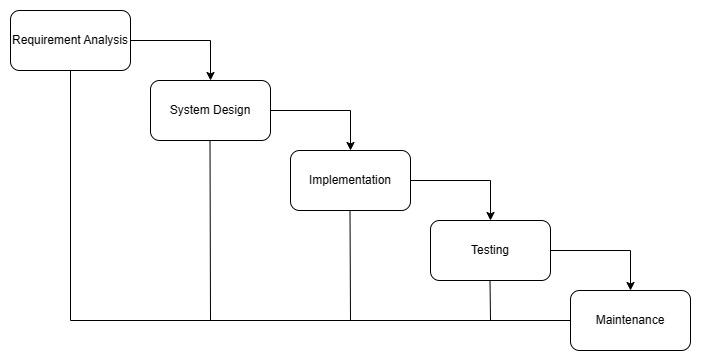
\includegraphics[width=9cm]{contents/chapter-2/waterfall_fig.png}
	\caption{Tahapan dalam metode SDLC \textit{waterfall}}
	\label{Fig:Waterfall_step}
\end{figure}

Metode Waterfall memiliki kelebihan dan kekurangan. 
Metode Waterfall merupakan metode yang mudah dipahami dan digunakan, terutama oleh \textit{developer} 
pemula. 
Metode Waterfall cocok digunakan untuk mengembangkan \textit{software} yang memiliki 
\textit{requirement} yang jelas dan cenderung tidak akan mengalami perubahan \textit{requirement} 
di tengah proses pengembangan. Metode ini juga cocok digunakan pada \textit{project} kecil 
yang memiliki risiko yang rendah. Metode ini tidak cocok digunakan 
untuk mengembangkan \textit{software} yang memiliki risiko yang tinggi karena 
metode ini tidak memiliki mekanisme untuk mengatasi perubahan \textit{requirement} 
di tengah proses pengembangan. Metode ini juga tidak cocok digunakan untuk 
mengembangkan \textit{software} yang memiliki \textit{requirement} yang tidak jelas. 
Hal ini dikarenakan metode ini tidak memiliki tahapan untuk melakukan analisis 
\textit{requirement} yang mendalam. 

\subsubsection{Metode SDLC Agile}
Metode \textit{agile} adalah metode SDLC yang paling fleksibel. Metode ini terdiri dari 
beberapa tahapan yang dapat dilakukan secara berulang-ulang atau bersifat \textit{iterative}. 
Terjadinya pengulangan tahapan biasanya disebabkan oleh sistem yang dikembangkan memiliki 
\textit{requirement} yang belum jelas atau dapat berubah sewaktu-waktu. Metode Agile 
berfokus pada adaptabilitas, fleksibilitas, dan kemampuan untuk bergerak dengan cepat, sesuai dengan 
namanya, yaitu \textit{agile} yang berarti lincah. Gambar \ref{Fig:Agile_step} merupakan 
lustrasi bagaimana metode Agile pada \textit{software development life cycle} (SDLC).

\begin{figure}[h]
	\centering
	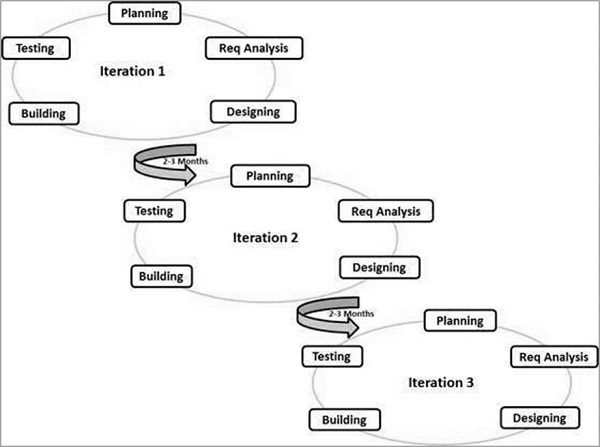
\includegraphics[width=9cm]{contents/chapter-2/sdlc_agile_model.jpg}
	\caption{Tahapan dalam metode SDLC \textit{Agile}\cite{noauthor_sdlc_nodate}}
	\label{Fig:Agile_step}
\end{figure}

Gambar \ref{Fig:Agile} menunjukkan tahapan-tahapan dalam metode \textit{agile}. 
Metode ini cocok digunakan untuk mengembangkan \textit{software} yang memiliki 
\textit{requirement} yang tidak jelas dan dapat berubah sewaktu-waktu. Metode ini 
juga cocok digunakan untuk mengembangkan \textit{software} yang memiliki risiko yang 
tinggi. Hal ini dikarenakan metode ini memiliki mekanisme untuk mengatasi perubahan 
\textit{requirement} di tengah proses pengembangan. Metode ini juga cocok digunakan 
untuk mengembangkan \textit{software} yang memiliki \textit{requirement} yang jelas. 
Metode ini tidak cocok digunakan untuk mengembangkan \textit{software} yang memiliki 
risiko yang rendah karena metode ini memiliki tahapan yang berulang-ulang dan 
membutuhkan waktu yang lebih lama dibandingkan dengan metode \textit{waterfall}. 
Metode ini juga tidak cocok digunakan untuk mengembangkan \textit{software} yang 
memiliki \textit{requirement} yang tidak jelas. Hal ini dikarenakan metode ini tidak 


\section{Analisis Perbandingan Metode}

% Di dalam tinjauan pustaka hasil akhirnya adalah analisis secara kualitatif atau pun secara kuantitatif kelebihan dan kekurangan metode jika dikaitkan dengan masalah, batasan-batasan masalah dan solusi yang dinginkan. Analisis kuantitatif tidak wajib teapi mempunyai nilai tambah di dalam tugas akhir saudara. Bagian ini menjelaskan kenapa metode tersebut dipilih dan uraikan dengan lebih jelas metode pelaksanaan tugas akhir yang ingin Anda lakukan. 

Pada bagian ini, akan dilakukan perbandingan metode-metode untuk mengembangkan aplikasi web, 
yang akan digunakan untuk mengembangkan sistem informasi penelitian dan pengabdian kepada 
masyarakat. Pemilihan metode didasarkan pada kompleksitas dan ukuran aplikasi, fleksibilitas 
, waktu, jumlah anggota tim, dan sebagainya. 

Seperti yang telah disebutkan pada bagian 2.2.7 mengenai metode pengembangan \textit{software}, 
metode \textit{waterfall} dan metode \textit{agile} merupakan dua dari beberapa metode 
pengembangan \textit{software} yang dapat digunakan. 

Keduanya memiliki kelebihan dan 
kekurangan masing-masing dan cenderung saling bertolak belakang. Metode \textit{waterfall} 
memiliki tahapan yang berurutan dan sekuensial, sehingga cocok digunakan untuk mengembangkan 
\textit{software} yang memiliki \textit{requirement} yang jelas dan cenderung tidak akan 
mengalami perubahan \textit{requirement} di tengah proses pengembangan. Metode \textit{agile} 
memiliki tahapan yang dapat dilakukan secara berulang-ulang atau bersifat \textit{iterative}, 
sehingga cocok digunakan untuk mengembangkan \textit{software} yang memiliki \textit{requirement} 
yang tidak jelas dan dapat berubah sewaktu-waktu. 